\documentclass[12pt]{third-rep}

%% Any characters from a % to the end of line are comments.

%% The third-rep class and this starter kit were written by 
%% Graham Gough <graham@cs.man.ac.uk>
%% If you have any comments or questions regarding this document,
%% please post them to the local newsgroup man.cs.tex.

%% This skeleton report is organised as a master file called
%% report.tex which then includes files for individual parts including
%% abstract.tex, chapter1.tex, chapter2.tex, chapter3.tex and
%% appendix1.tex.  

%% The third-rep style is a locally created style based on the
%% standard LaTeX report style. If you really want to have a look at
%% it, its source can be found in
%% /usr/local/share/texmf/tex/latex/mancs/third-rep.cls
%%
%% More information about LaTeX in general and the local setup in
%% particular can be found on the web at 
%% http://www.cs.manchester.ac.uk/software/tex/
%%
%%%%%%%%%%%%%%%%%%%%%%%%%%%%%%%%%%%%%%%%%%%%%%%%%%%%%%%%%%%%%%%%%%%%%%%%
%%
%% This is an example of how you load extra packages.
%% Some packages are already loaded in the third-rep class

\usepackage{url} % typeset URL's sensibly
\usepackage{amsmath}
\usepackage{pslatex} % Use Postscript fonts
\usepackage[utf8]{inputenc}
\usepackage[T1]{fontenc}
\usepackage{listings}

\usepackage{color}
 
\definecolor{dkgreen}{rgb}{0,0.6,0}
\definecolor{gray}{rgb}{0.5,0.5,0.5}
\definecolor{mauve}{rgb}{0.58,0,0.82}
 
\lstset{ %
  language=Java,                % the language of the code
  basicstyle=\footnotesize,           % the size of the fonts that are used for the code
%  numbers=left,                   % where to put the line-numbers
%  numberstyle=\tiny\color{gray},  % the style that is used for the line-numbers
%  stepnumber=2,                   % the step between two line-numbers. If it's 1, each line 
                                  % will be numbered
  numbersep=5pt,                  % how far the line-numbers are from the code
  backgroundcolor=\color{white},      % choose the background color. You must add \usepackage{color}
  showspaces=false,               % show spaces adding particular underscores
  showstringspaces=false,         % underline spaces within strings
  showtabs=false,                 % show tabs within strings adding particular underscores
%  frame=single,                   % adds a frame around the code
  rulecolor=\color{black},        % if not set, the frame-color may be changed on line-breaks within not-black text (e.g. commens (green here))
  tabsize=2,                      % sets default tabsize to 2 spaces
  captionpos=b,                   % sets the caption-position to bottom
  breaklines=true,                % sets automatic line breaking
  breakatwhitespace=false,        % sets if automatic breaks should only happen at whitespace
  title=\lstname,                   % show the filename of files included with \lstinputlisting;
                                  % also try caption instead of title
  keywordstyle=\color{blue},          % keyword style
  commentstyle=\color{dkgreen},       % comment style
  stringstyle=\color{mauve},         % string literal style
  escapeinside={\%*}{*)},            % if you want to add a comment within your code
  morekeywords={*,...}               % if you want to add more keywords to the set
}
%% The best way to latex just one chapter is to uncomment lines such as
%% the next:
%\includeonly{chapter1}

%% This defines the title (the \\ forces a line break)
\title{Text Mining Twitter for Software\\
  and User Perception}
%% and author
\author{Tariq Patel}
%% and supervisor
\supervisor{Dr. Goran Nenadic}
%% and the year of the report
\reportyear{2012}

%% this defines the file that contains the text of the abstract, there
%% must be one of these by the time you submit your report.
\abstractfile{abstract.tex}

%% this defines the file that contains the acknowledgements (it can be
%% omitted if you don't feel like thanking anyone
%\thanksfile{merci.tex}

%% End of preamble, the actual document starts here
\begin{document}

%% This actually creates the title and abstract pages
\dotitleandabstract

%% Generate contents etc
\tableofcontents
\listoffigures
\listoftables
\lstlistoflistings

%% These include the actual text
\chapter{Introduction}
\label{cha:intro}

\section{Motivation}
The success of a piece of software is based largely upon user opinion. Gathering such information is conventionally done through means of surveying groups of users. However, in the days of social media, people generally express their opinions on popular social networks or microblogging sites such as Facebook and Twitter. This means it is now much easier for companies to receive and collect feedback on products they have developed by monitoring these networks.

Twitter has been at the core of many data mining projects in recent years and this is due to the sheer amount of data produced on a daily basis. Twitter users now post in excess of 340 million tweets every day~\cite{twitterblog} and as such Twitter provides a massive corpus\footnote{A collection of documents} for opinion mining and sentiment analysis.
%MORE

\section{Aim}
\label{sec:aim}
By text mining Twitter posts for software, users may be able to discover new tools or programs they have not come across before, as well as see reviews by other users.

The aim of this project is to develop a system that text mines Twitter posts to find software or software development tools that have been mentioned by its users and to discover the general sentiment of users towards these software. This system will henceforth be called \textbf{SWOT} - Software on Twitter.

\section{Challenges}
There are many challenges facing Natural Language Processing(NLP)-oriented projects.

With the millions of tweets posted every day on Twitter, one can safely presume that many of these will have no relevance to software or any of the other desired information. As such it will be vital to ensure only the most relevant tweets are extracted from Twitter for analysis so as not to waste resources.

Another issue is the world-wide nature of the Internet and microblogging networks like Twitter. This means that several tweets will not be in English and for this reason it would be more difficult to extract features from these tweets. To counter this, it will be necessary to filter tweets not only based on key words but also on their language.

A major issue in NLP research is that of text message shorthand. In a formal document, this problem becomes somewhat irrelevant due to proper usage of Standard English. However, when working with the Twitter platform, the service's 140 character limitation on tweets means users are generally more likely to abbreviate their text and this allows for a lot of ambiguity in the context of each word, and variability in how users may say the same thing.
% EXAMPLE HERE
%AGGREGATION?

\section{Objectives}
In order to successfully complete a project of this magnitude, the task at hand must be split into smaller steps.  These objectives are shown with their complexities and priorities in Table~\ref{objectives}.

\begin{table}
\begin{center}
\begin{tabular}{|r|c|}\hline\hline
&Task\\\hline
1&Collect and filter tweets by keyword\\
2&Feature extraction\\
3&Analyse tweet sentiment\\
4&Structure and integrate data\\
5&Visualise data through GUI\\
6&Evaluate the system\\\hline\hline
\end{tabular}
\end{center}
\caption{Complexity and priority of project objectives}\label{objectives}
\end{table}

\subsection{Collect and Filter Tweets by Keywords}
Collecting tweets is a core task in this project as all the work will be based on tweets stored in a database. Filtering through these is a relatively simple task in that it can be done using Twitter's APIs, but there are some complexities in ensuring they are all relevant.

The main idea at this stage is to collect tweets based on a set of keywords and software names, programming languages, or company names stored in a dictionary, in order to retrieve relevant, software-related tweets.

\subsection{Feature Extraction}
Feature extracting is the core functionality set out to be achieved in this project. Using rule-based text mining techniques, the aim of this task will be to retrieve up to eight features from every tweet, which are shown in Table~\ref{features}. Tweets will generally not contain all eight features and so the application cannot be expected to fill all of these fields for every tweet.

\begin{table}
\begin{center}
\begin{tabular}{|r|l|}\hline\hline
&Feature\\\hline
1&Software name\\
2&Software version\\
3&Company or developer\\
4&Programming language\\
5&Operating system\\
6&Price\\
7&Relevant URLs\\
8&Tweet sentiment\\\hline\hline
\end{tabular}
\end{center}
\caption{Features to be extracted from tweets}\label{features}
\end{table}

% Remove this?
These features have been selected in order to find useful information from tweets to be displayed to users. The \textbf{software name} is of course vital, in that this discovery is the main purpose of the project. The \textbf{version} of this software is important because major changes may have been made over the course of a few releases and so it is necessary to note which release people are referring to. The \textbf{company name} is not a major feature, however it may be interesting to know who developed a certain piece of software. It may also be used in a different scenario where a user of this system wishes to find public sentiment towards a company as opposed to some specific software. The \textbf{programming language} feature ideally signifies the language or languages in which the found software was developed in. However, as with the company field, this may be used to find sentiment towards specific programming languages or practices. The \textbf{operating system} field works in a similar fashion, in that its expected use is to find the operating systems upon which the found software runs, but it can also be used to find the sentiment towards a specific operating system. \textbf{Price} and \textbf{URL} extraction are geared towards retrieving information about the product for the user. 

\subsection{Analyse Tweet Sentiment}
Sentiment analysis is another of the more important tasks in this project. This is where tweets are analysed for subjectivity, i.e. whether the tweet is positive, negative or neutral. The \textbf{tweet sentiment} feature to be extracted aims to find the general sentiment towards a piece of software, and will be used in the aggregation process in the final stages when trying to establish public perception of the software.

\subsection{Structure and Integrate Data}
The data needs to be structured and aggregated to be able to provide any meaningful output for the user.

\subsection{Visualise Data Through GUI}
Visualising the data is a fairly low priority task in that the system first needs to gather the information. This project centres more around the core back-end development than user experience and as such only a simple user interface is needed in its initial stages.

\subsection{Evaluate the System}
The final evaluation of the produced system will be key in determining the success of this project. The system will be evaluated on the basis of the accuracy of retrieved results, the relevance and novelty of information, and general usability.

\section{Report Structure}
This report documents the implementation of a text mining system that is set out to achieve the previously stated goals. The remainder of this report has been split into 6 chapters.
Chapter~\ref{cha:background} details the general background of this project and previous work in the area.
Chapter~\ref{cha:design} goes into the design of the software implementation including use case analysis, the architecture of the system and the software engineering methodologies used.
Chapter~\ref{cha:impl} describes the process of implementing each stage of the project and goes into details of how specific aspects such as the Twitter API integration and feature extraction work.
Chapter~\ref{cha:results} illustrates the results and final outcomes of the project with any meaningful information gained.
Chapter~\ref{cha:eval} provides the general evaluation of the finished project, also outlining the successes and failures of the task at hand.
Finally, Chapter~\ref{cha:conclusion} concludes the author's conclusions of the project, with suggestions for further work.

\chapter{Background}
\label{cha:background}
This chapter provides an overview of the text mining field along with previous work in the area and all necessary background information required to understand the major tasks involved in this project. This is followed up with an overview of the different APIs provided by Twitter to work with their platform.

\section{Text Mining}
\label{sec:textmining}
The information available in the world is growing exponentially, and the majority of this information is unstructured (widely estimated at roughly 80\%)~\cite{Grimes08}. This is where text mining comes in, also referred to as Knowledge Discovery from Text (KDT).
``Text mining is the process of extracting interesting information and knowledge from unstructured text''~\cite{hotho-etal-ldv-2005}. Its applications tend to work in two steps, first using an Information Retrieval (IR) application to narrow the search space, and then they extract significant parts of the retrieved texts~\cite{Polajnar2006}. This general process usually involves structuring a source text by means of parsing and other linguistic analysis, then finding patterns in this structured data and then interpreting this output. An example of the text mining process can be seen in Figure~\ref{fig:tm}.

Text mining is fundamentally different from standard web searching in that web searches rely primarily on information that is already known. On the other hand, the goal of text mining is to discover interesting, previously unknown information~\cite{Gupta_Lehal_2009}.
There is one key issue about text mining; natural language is used by humans for communication and recording information, while computers are incapable of interpreting natural language. Humans are naturally able to find linguistic patterns in text and understand the semantics of what is being said. Computers, on the other hand, face difficulties in interpreting variations in written text through spelling, colloquialism and also the general context of the text. Nonetheless, computers are much more capable of processing large datasets at very high speeds, particularly in comparison to humans. 
Thus, the objective of text mining is to create an application that is able to apply human-defined rules to large datasets  in order to extract linguistic patterns. Machine learning techniques could also be applied, however these are not in the scope of the project as a rule-based approach has been taken.

\begin{figure}[t]
\begin{center}
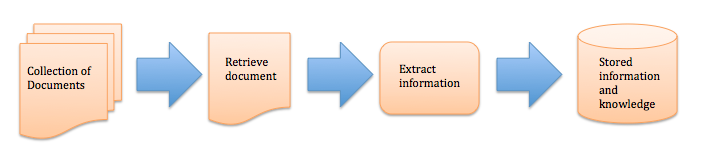
\includegraphics[width=15cm]{tm}
\end{center}
\caption{The text mining process \cite{Gupta_Lehal_2009}}
\label{fig:tm}
\end{figure}

\subsection{Information Retrieval}
Information Retrieval (IR) is the process of retrieving textual documents which may contain the answers to questions but the process itself does not answer these questions~\cite{Hearst:1999}. Information retrieval is fundamentally a web search working off user queries representing an information need. The process works by searching a collection of documents, and then retrieving those matching a user query depending on relevance. The approach to calculating relevance is dependent upon the actual IR engine itself. Generally, this works on the frequency of specific key terms in each of these documents, and usually assigns a relevance rank to each one. This allows for improved results through sorting, particularly when restrictions are placed on the number of results to return.

The IR tasks in this project will mainly be carried out on Twitter's systems, and as such, besides the core concept of IR, its internal specifics are not in the scope of this report.

\subsection{Natural Language Processing}
Natural Language Processing (NLP), in the scope of this project, is the process of extracting information from natural language~\cite{Healey98}, that is, any language written or spoken by humans. This involves parsing and processing unstructured text to be able to gain meaningful knowledge from it. Nowadays natural language processing is done using machine learning techniques. However, in the past, implementations were based on large sets of coded rules. These rules are used to define certain linguistic features in the text in order to understand the semantics behind it. NLP is a major field of research at present and also has applications in both information retrieval and extraction.

There are many methods involved in NLP tasks and some of these will now be further explored.

\subsubsection{Tokenisation}
Tokenisation is the process of splitting a stream of text into singular words or phrases, otherwise known as tokens. These tokens usually form the basis of further NLP processing. While it can be a straightforward process when using Standard English, the definition of a word, from the tokeniser's point of view, can be somewhat ambiguous. This is particularly true when considering the use of apostrophes. Figure~\ref{fig:tokenisation} shows an example of the different ways of tokenising the word \emph{don't}.

\begin{figure}[h!]
  \centering
  \setlength{\unitlength}{0.0125in}
\begin{picture}(80,105)( -20, 0)
\thicklines
\put(0,100){\framebox{don't}}

\put(0,80){\framebox{dont}}

\put(0,60){\framebox{don}}
\put(30,60){\framebox{'t}}

\put(0,40){\framebox{don}}
\put(30,40){\framebox{t}}

\put(0,20){\framebox{do}}
\put(25,20){\framebox{n't}}

\put(0,0){\framebox{do}}
\put(25,0){\framebox{nt}}
\end{picture}

  \caption{The different ways of tokenising the word \emph{don't}
    \label{fig:tokenisation}}
\end{figure}

These variations can be problematic in terms of the results being output for certain user queries. For example, in the case of these differing tokenisations of \emph{don't}, a user search for the word \emph{don} would return a positive match twice, but should be negative in its actual context. The importance of normalisation is highlighted when tokenising tweets because a lot of users do not use apostrophes, either due to ease when typing, or in order to reduce the number of characters being used. Thus, varying spellings of the terms should not be tokenised differently.

\subsubsection{Normalisation}
Once text has been tokenised, these words may need normalising. Normalisation accounts for the several variations in spelling. For example, if you want to search for \emph{Mozilla~Firefox} you would want an IR engine to return not only documents containing the exact query but also those containing terms such as \emph{Firefox}, \emph{firefox} and \emph{mozilla~firefox}. Failing to normalise terms would obviously yield fewer results, or in the case of information extraction, it may suggest that \emph{Mozilla~Firefox} and \emph{mozilla~firefox} are two different entities. Thus, normalisation is required to successfully map equivalent classes of terms.

\subsubsection{Stop Word Filtering}
Stop words are very commonly used words like \emph{a}, \emph{I} and \emph{the} that do not bear any specific meaning on their own. By creating a list of these terms, a \emph{stop list}, a natural language parser can remove these terms from the source text as they hold little or no value in matching queries to documents. In modern systems, however, stop lists are not widely used as they provide little gain in terms of efficiency~\cite{manning2008}.

\subsubsection{Part of Speech Tagging}
Part of Speech (POS) tagging is a process typically carried out after tokenisation. Its task is to assign tags to words, for their corresponding grammatical parts of speech, based on both the word's definition, and its context. This is essentially identifying words as nouns, verbs, adjectives, etc.

However, the process is more complicated than it may first seem. The main issue is that most words do not just have one part of speech, they can have many. For example, \emph{can} could be a noun or a verb, depending on the context it is being used in. Thus, when tagging words, it is important to analyse a whole phrase or sentence. Analysing a word out of context could have significant repercussions. In the context of this project, taking the Microsoft software \emph{Paint} as an example, if someone were to tweet:
\begin{quote}
Microsoft Paint has seen some major improvements in its latest release!
\end{quote}
This would differ from, say,
\begin{quote}
Paint something now.
\end{quote}
where \emph{paint} is being used as an imperative verb. In the first example, seeing that \emph{Paint} is followed by \emph{seen}, a verb, suggests it is unlikely \emph{Paint} is being used as verb.  This would be the difference in this project between discovering a piece of software and totally missing it, and thus highlights the importance of context and semantics when analysing text.

\subsubsection{Stemming and Lemmatisation}
Documents contain many different derivations of words, such as \emph{normalise} and \emph{normalisation}, and differing forms of the same word due to its usage or tense, for example, \emph{walked} or \emph{walking}. An information extraction tool should ideally see these as somewhat equivalent terms; this is where stemming and lemmatisation come in. The following example, taken from \cite{manning2008}, shows how these techniques should map text:

\begin{quote}
am, are, is \begin{math}\Rightarrow\end{math} be 
\newline
car, cars, car's, cars' \begin{math}\Rightarrow\end{math} car
\newline
\newline
the boy's cars are different colors  \begin{math}\Rightarrow \end{math}
\newline
the boy car be differ color
\end{quote}

Stemming is an heuristic process hoping to achieve this goal by simply building basic forms of words by removing affixes like a plural `s' from nouns or the `ing' from verbs~\cite{hotho-etal-ldv-2005}. However, these are not always correct terms. Lemmatisation on the other hand utilises a more sophisticated approach in that it uses a vocabulary and morphological analysis of words, in order to return to the true base form of a word that may be found in a dictionary. This process, however, is much more complex and time-consuming than the former, and stemming may be sufficient for some applications.

\subsection{Information Extraction}
The goal of Information Extraction (IE) is to extract specific data from a given corpus. IE can be defined as the task of automatically extracting structured information from unstructured or semi-structured machine-readable documents, generally done through the use of NLP techniques.

In structured texts, information extraction can be fairly straightforward, as labels or tags may delimit strings that need to be extracted~\cite{soderland99}. However, in unstructured texts, information is not as clearly understandable by computers and so IE requires techniques from other fields such as machine learning, statistical analysis or those previously discussed from natural language processing.

Typical IE tasks include the following:

\subsubsection{Named Entity Recognition}
The aim of Named Entity Recognition (NER) is to annotate a source text with markup tags in order to classify strings representing predefined categories such as names, companies, locations, dates and times. For example,
\begin{quote}
Cook named new Apple CEO.
\end{quote}
would yield the following annotations.
\begin{quote}
<ENAMEX TYPE="PERSON">Cook</ENAMEX> named new
\newline
<ENAMEX TYPE="ORGANIZATION">Apple</ENAMEX> CEO.
\end{quote}

This example is using the \emph{ENAMEX} tags defined at the Message Understanding Conference (MUC) in the 1990s~\cite{grishman96muc}. From the source text it can be seen that \emph{Cook} has been identified as a person and \emph{Apple} as an organisation and structures this text in doing so.

\subsubsection{Relationship Extraction}
This works with entity extraction in that it works to identify relations between entities. Using the previous example, the relationship extraction process should be able to identify that,
\begin{quote}
PERSON named new ORGANISATION CEO.
\end{quote}

% OTHER SUB TASKS?

\section[Sentiment Analysis]{Sentiment Analysis and Opinion Mining}
Sentiment analysis, also known as opinion mining, refers to the NLP application of extracting subjective information in source texts. There are two use cases for sentiment analysis. The first of these is determining whether a text is subjective or objective, that is, whether the statement is factual or opinionated. This scenario is not currently in the scope of the project and leads to the second use case; sentiment analysis also aims to classify the \emph{polarity} of a given text~\cite{Pang+Lee}. This, to the basic level, involves determining whether an expressed opinion is positive, negative or neutral, but can also be extended to more complex emotions such as happy or sad.

Opinion mining can be done using a weighting system. This method assigns a positive or a negative weighting on a given scale such as -3 to +3. These are applied for each word in the text that relates to the core entity. The text is then given a total score which determines its polarity, and also the strength of the sentiment. In simpler systems the scale may only be from -1 to +1, essentially opting to ignore the strength of the sentiment and just asking for the general sentiment of the text.

% More?

\section{Evaluation Measures}
In text mining, there are several ways of evaluating the accuracy of a system. Before discussing the different measures, few key prediction outcomes must first be defined.

\textbf{True Positive $tp$} - an entity is predicted to have a certain property, and it in fact does

\textbf{False Positive $fp$} - an entitiy is predicted to have a certain propery but it does not

\textbf{True Negative $tn$} - an entity is correctly predicted to not have a certain property

\textbf{False Negative $fn$} - an entity is incorrectly predicted to not have a certain property

The main measures to be used in the scope of this project are described below.

\subsection{Precision}
Precision is the fraction of retrieved documents that are relevant to the search. This is the number of correct results divided by the total number of results.
\begin{quote}
$\mathrm{Precision}=\frac{tp}{tp+fp}$
\end{quote}

\subsection{Recall}
Recall is the fraction of relevant documents that are successfully retrieved. This means it is a measure of the number of correct results that were retrieved out of all of the results that should have been returned. This is the number of correct results returned divided by the total number of all correct results.
\begin{quote}
$\mathrm{Recall}=\frac{tp}{tp+fn}$
\end{quote}

\subsection{Specificity}
Specificity is also known as the True Negative Rate. It is the measure aiming to find the accuracy of a system in identifying negative results. This is the number of identified negative results divided by the total number of negative results.
\begin{quote}
$\mathrm{Specificity}=\frac{tn}{tn+fp}$
\end{quote}

\subsection{F-Measure}
The F-measure combines precision and recall to find a weighted average of the two measures.
\begin{quote}
$F = 2 \cdot \frac{\mathrm{precision} \cdot \mathrm{recall}}{\mathrm{precision} + \mathrm{recall}}$
\end{quote}

\section{Twitter Mining}
There has been several previous works on text mining Twitter posts, however, the bulk of these have focussed primarily on biomedicine and the financial sector. These works have shown the potential in Twitter has for providing valuable knowledge and information it is felt that software is a new area of interest where Twitter has not previously been used to analyse public opinion. Twitter's low character limit means users have to express their opinions explicitly and encourages the use of emoticons, such as :) or :(, which have been shown to work very well in sentiment analysis~\cite{Read:2005}.

% MORE

\section{Twitter API}
Twitter provides three public APIs for developers to access their massive corpus of data. These are the REST, Search and Streaming APIs, and shall now be further explored.

\subsection{Search API}
The Search API is the simplest tool provided by Twitter. This API is designed to allow users to query for Twitter content and works very much like the search bar found on the Twitter website itself. This content may include a set of tweets with specific keywords or tweets to, from or mentioning a specific user. A simple search would yield up to 1500 of the latest tweets in the last 7 days, which have been cached over a 60 second period. There are, however, restrictions on the rate at which programs can utilise this API~\cite{twitter}.

\subsection{REST API}
The REST API enables programs to access more of the core Twitter functions. This API retrieves not only the information taken from the Search API but also allows building timelines and retrieves more specific user information such as the user's name, profile avatar, tweet count and the number of followers and friends they have. The REST API also allows programs to post on Twitter and carry out other functions like retweeting or favouriting tweets. These extra functions, however, are not required in this project.

\subsection{Streaming API}
Twitter's Streaming API is a real-time sample of all public tweets posted on the sample. It allows filtering in various ways such as user id, keywords or even random sampling, and is regarded as the default option for data mining operations. This is because the Streaming API allows a long-lived HTTP connection unlike the other APIs and as such, programs can constantly remain connected so as to retrieve a running stream of tweets, as the name itself suggests. This removes the overheads associated with reconnecting every time you want to make a query and the API also removes all rate limitations so there is no worry of exceeding your quota. Unlike the other APIs, programs must be authenticated to use the Streaming API.


\section{Summary}



\chapter{Design}
\label{cha:design}


%\begin{table}
%\begin{center}
%\begin{tabular}{|r|c|c|c|}\hline\hline
%&Task&Complexity&Priority\\\hline
%1&Collect and filter tweets by keyword&Simple&High\\
%2&Feature extraction&Complex&High\\
%3&Analyse tweet sentiment&Intermediate&Medium\\
%4&Structure and integrate data&Intermediate&High\\
%5&Visualise data through GUI&Intermediate&Low\\
%6&Evaluate the system&Complex&High\\\hline\hline
%\end{tabular}
%\end{center}
%\caption{Complexity and priority of project objectives}\label{objectives}
%\end{table}



This chapter details the overall design of the system to be developed in this project. The software engineering methodology to be used will first be discussed, along with use cases, requirements and the architecture of the system. This will be followed up with notes on the class and database design diagrams. The decisions made with regards to some design choices will also be discussed in more detail.

\section{Software Engineering Methodology}
The software engineering methodology used in developing an application can have many effects on its final outcome. The development of this system will be carried out using principles taken from continuous integration and agile methods such as feature-driven development. There is always a working code repository available for deployment, and all new features to be implemented are to be worked on in clones of said repository. Upon completion of these minor implementations, they are tested to ensure everything is working correctly and assuming there are no issues, the changes are merged into the base repository. This methodology assures developers that if any major issues arise due to recent changes, they will be able to discard all changes and restart if they feel debugging would be a longer process. This ultimately allows for a faster development cycle and provides rigorous testing throughout the implementation process. This development methodology also allows for frequently changing requirements which is to be expected in any development task.

\section{Use Cases}
\label{sec:uc}
To serve as a reminder, the aim of this project is to develop a system, SWOT, that text mines Twitter posts to find software or software development tools that have been mentioned by its users and to discover the general sentiment of users towards these software. 

In order to attain this goal, SWOT must satisfy four uses cases, as seen in Figure~\ref{fig:uc}, which have been described below.

\begin{figure}[h]
\begin{center}
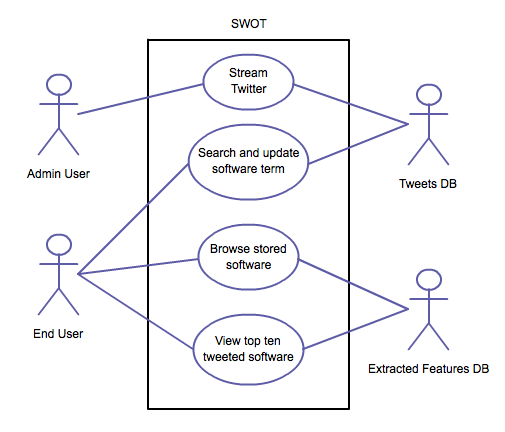
\includegraphics[width=12cm]{uc}
\end{center}
\caption{Use cases for SWOT}
\label{fig:uc}
\end{figure}

\subsection[Use Case 1]{UC1 - Stream Twitter}
\label{sec:uc1}
The first use case for the system requires a tool capable of continuously monitoring public tweets and storing these in a database. These tweets should be filtered by language and relevance, that is, tweets should be related to software. These tweets need to be filtered by language to counter any issues faced in the feature extraction stage due to the complexities involved in NLP. This use case is targetted for use by an administrator as the process should be running constantly in the background.

\subsection[Use Case 2]{UC2 - Search and Update Software Term}
\label{sec:uc2}
SWOT's second use case requires the ability to search Twitter for tweets concerning user-specified key terms. This is ideally the name of some software that may or may not already be present in the database of extracted software and features. In the case where the software is not already present, it will now be added upon finding tweets. Where the software already exists in the database, the search will still be carried out in order to retrieve more recent tweets matching the search query, in order to update the stored data.

\subsection[Use Case 3]{UC3 - Browse Stored Software}
\label{sec:uc3}
The third use case involves allowing users to view the information stored in the database of extracted software and features. This should be displayed in the form of charts displaying the sentiment of tweets and all relevant information found alongside it.

\subsection[Use Case 4]{UC4 - View Top Ten Tweeted Software}
\label{sec:uc4}
The final use case for SWOT requires displaying to users the software tools that have been mentioned most often on Twitter. Users should then also be able to carry out use cases 2 and 3 with these tools.

\section{General Architecture}
The system design follows a 3-stage approach, these being tweet retrieval, feature extraction and visualisation for users. These stages are shown in the general archicture model displayed in Figure~\ref{fig:general}. These will be further explored in Sections~\ref{sec:arc1}, \ref{sec:arc2} and \ref{sec:arc3} respectively.

\begin{figure}[h]
\begin{center}
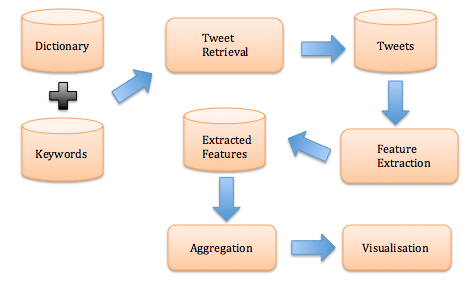
\includegraphics[width=10cm]{design}
\end{center}
\caption{General architecture of the SWOT system}
\label{fig:general}
\end{figure}

\subsection{Retrieving Tweets}
\label{sec:arc1}
The first stage involves retrieving tweets from Twitter. The design for this stage follows the same concepts for each of the use cases defined. This can then be split further as seen in Figure~\ref{fig:phase1}. The program should retrieve a set of search terms from a dictionary along with some keywords that may be associated with software. This dictionary consists of a list of software, companies, operating systems and programming languages. The full list of keywords and dictionary items can be seen in Table~\ref{tbl:keywords} and Appendix~\ref{app:dictionary} respectively. The respective counts for each of these types of items is shown in Table~\ref{tbl:dict_types}.
These are to be used to form a request for tweets from Twitter. Twitter will respond with the corresponding tweets and data, which are to be checked for language, to ensure they are in English. The remaining set of English tweets are then to be further parsed to extract the required information for storing these tweets in the database.

\begin{table}[h]
\begin{center}
\begin{tabular}{|l|l|l|}\hline
alpha&api&app\\\hline
beta&game&mac\\\hline
pc&release&sdk\\\hline
software&source code&version\\\hline
\end{tabular}
\end{center}
\caption{List of keywords}
\label{tbl:keywords}
\end{table}

\begin{table}[h]
\begin{center}
\begin{tabular}{|l|r|}\hline\hline
\textbf{Type}&\textbf{Count}\\\hline
Software&389\\
Operating System&12\\
Company&25\\
Programming Language&448\\
Keywords&12\\\hline
\textbf{Total}&\textbf{886}\\\hline\hline
\end{tabular}
\end{center}
\caption{Number of terms for dictionary types}
\label{tbl:dict_types}
\end{table}

\begin{figure}[h]
  \centering
  \setlength{\unitlength}{0.0125in}
\begin{picture}(300,35)(95,730)
\thicklines
\put(0,740){\framebox(75,20){Filter terms}}
\put(75,750){\vector( 1, 0){ 20}}
\put(95,740){\framebox(75,20){Twitter API}}
\put(170,750){\vector( 1, 0){ 20}}
\put(190,740){\framebox(110,20){Language detection}}
\put(300,750){\vector( 1, 0){ 20}}
\put(320,740){\framebox(80,20){Parse response}}
\put(400,750){\vector( 1, 0){ 20}}
\put(420,740){\framebox(75,20){Store in DB}}
\end{picture}

  \caption{Design for tweet retrieval
    \label{fig:phase1}}
\end{figure}

This returned information will be stored in a relational database and its design is shown below in Figure~\ref{fig:db}. Tweets will not be stored alone but also with simple user information to allow for future user profiling for a more targetted approach to tweet retrieval. The actual tweet information to be stored is its id on the Twitter platform - allowing for cases where users delete their tweets - its text content, time of creation, user id and the keyword used to find it, where one was used. There will also be fields for sentiment, i.e. positive, negative or neutral, and sentiment strength, where weightings have been used. These fields should default to \texttt{NULL} as their values will be computed at a later time. Finally, there is a \emph{tagged} boolean flag which signifies the given tweet has been processed, and the feature extraction process has been carried out on it. This is to work in conjunction with the \emph{found} boolean flag which indicates whether or not software has been found in the tweet. This is to be implemented in MySQL due to its simplicity, compatibility with the design and also because it is readily available on the university computers where data can be easily accessed both locally and remotely.

\begin{figure}[h]
\begin{center}
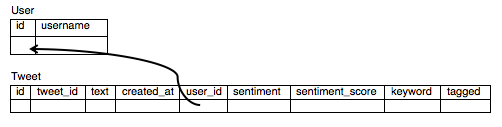
\includegraphics[width=12cm]{db}
\end{center}
\caption{Database design for storing tweets}
\label{fig:db}
\end{figure}

\subsection{Feature Extraction}
\label{sec:arc2}
The feature extraction stage will execute the task of extracting information from tweets. The aim at this stage is to extract the following features:

\begin{itemize}
\item \textbf{Software name} - This discovery is the main purpose of the project and as such is vital.
\item \textbf{Software version} - The version of the software is important because major changes may have been made over the course of a few releases, and so it is necessary to note which release people are referring to.
\item \textbf{Company name} -  This is not a major feature, however it may be interesting to know who developed a certain piece of software. It may also be used where a user of the system wishes to find public sentiment towards a company as opposed to some specific software.
\item \textbf{Programming language} - This feature ideally signifies the language or languages in which the found software was developed. However, as with the company field, this may be used to find sentiment towards specific programming languages or practices.
\item \textbf{Operating system} - Operating system (OS) extraction works similarly to company and programming language extraction in that its expected use is to find the operating systems upon which the found software runs, but it can also be used to find the sentiment towards a specific OS.
\item \textbf{Price} - This is geared towards retrieving information about the user.
\item \textbf{Relevant URLs} - URLs are also extracted for extra information.
\item \textbf{Tweet sentiment} - This is another important feature in terms of the overall project goals. The tweet sentiment aims to find the general sentiment towards a piece of software in a tweet. This will also be used in the final aggregation stages when trying to establish public perception of the software.
\end{itemize}

This will involve the stages described in \ref{sec:textmining} and its general design can be seen in Figure~\ref{fig:phase2}. The main aim of this stage is to take the tweets previously stored in the database and find the software mentioned in them.

\begin{figure}[h]
  \centering
  \setlength{\unitlength}{0.0125in}
\begin{picture}(300,200)( 50, 0)
\thicklines
\put(0,140){\framebox(110,20){Sentiment analysis}}
\put(110,150){\vector( 1, 0){ 20}}
\put(130,140){\framebox(100,20){URL extraction}}
\put(170,750){\line( 1, 0){ 10}}
\put(180,750){\line(0,-1){50}}

\put(300,750){\vector( 1, 0){ 20}}
\put(400,750){\vector( 1, 0){ 20}}



\put(130,140){\framebox(100,20){Price extraction}}
\put(130,140){\framebox(100,20){POS Tagging}}
\put(130,140){\framebox(100,20){Main features}}
\put(130,140){\framebox(100,20){Verify software}}


\end{picture}

  \caption{Design for feature extraction
    \label{fig:phase2}}
\end{figure}

Due to the volatile nature of the information being extracted from these tweets, this data should be stored in a NoSQL-type database, that is, a schema-less design that diverges from the traditional relational database model. As a result, there is no formal design for this database structure, however, it is required of the system to at this stage store any features it has managed to extract along with the key information associated with the tweet that had been stored in the tweet retrieval stage, such as its unique id and text content.

\subsection{Aggregation and Visualisation}
\label{sec:arc3}
The visualisation stage has the task of displaying all the gained information and knowledge to the user. Ultimately, it must also provide a graphical interface for users to interact with the system in order to perform their own searches.

There are two parts to this phase of project. Firstly, the data gathered must be \emph{aggregated} so that meaningful knowledge can ultimately be represented. Upon completing this task, a \emph{graphical user interface} must be designed for users to interact with the system, perform their own queries, and look at what information has been found.

\subsubsection{Aggregation}
Aggregating the results is the process of bringing together all of the different data sources for data on a single output entity such as a piece of software. This aggregated data can then be used easily by the GUI to display information to the user. In this project, this task will entail grouping the stored documents by software or other similar information such as company or operating system. Once this information has been retrieved, statistics and charts can be derived. The main task here is to create pie charts for each piece of software to show the sentiment of the tweets mentioning them. Other details include the most tweeted pieces of software.

\subsubsection{Graphical User Interface}
\label{sec:guid}
Upon the completion of the aggregation tasks, these charts and statistics need to be passed to a Graphical User Interface (GUI). The GUI of choice for this system is a web application, as opposed to a desktop application. This is a more extensible solution as changes would not need to be pushed out to all users.

There will be three actions for users to carry out on this GUI. These will relate to use case 2 of this system, as seen in Section~\ref{sec:uc2}. The first action to carry out will be searching for tweets posted on Twitter. A mockup of this action can be seen in Figure~\ref{fig:guiwire2}. Once these tweets have been retrieved from the Twitter Search API, they will be displayed on the web page, and in turn features will be extracted, and again displayed to the user.

After this, there will be an analysis page. This page will show a list of software or operating systems, from which a user can select to view charts displaying sentiment and a list of tweets. These charts will have been creating in the aggregation stage, but should be dynamically created. This page is shown in Figure~\ref{fig:guiwire3}.

Finally, once a number of tools, that is, software, operating systems etc. have been found in tweets, the home page should display a list of the most tweeted of these items. Clicking on an item in this list should offer the option of searching again for it, in order to update information, or to view its charts and sentiment information. This should look as the wireframe in Figure~\ref{fig:guiwire1}.

\begin{figure}[h]
\begin{center}
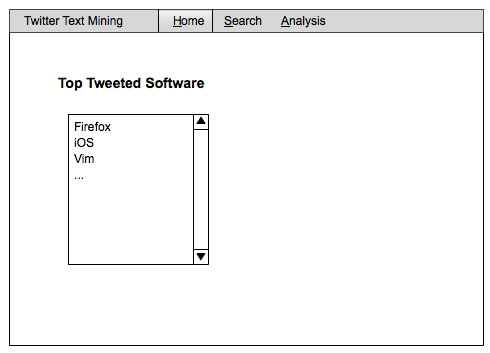
\includegraphics[width=10cm]{guiwire1}
\end{center}
\caption{A mockup of the website's home page}
\label{fig:guiwire1}
\end{figure}

\begin{figure}[h]
\begin{center}
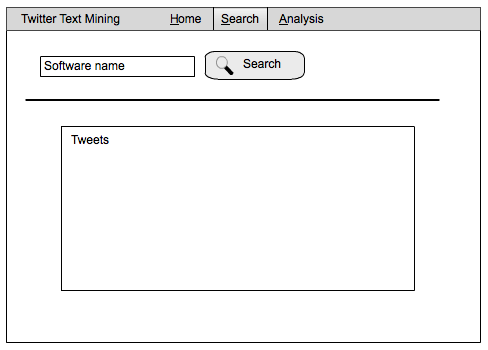
\includegraphics[width=10cm]{guiwire2}
\end{center}
\caption{A mockup of the website's search page}
\label{fig:guiwire2}
\end{figure}

\begin{figure}[h]
\begin{center}
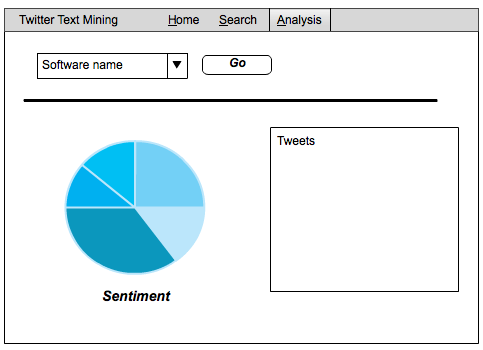
\includegraphics[width=10cm]{guiwire3}
\end{center}
\caption{A mockup of the website's analysis page}
\label{fig:guiwire3}
\end{figure}


\chapter{Implementation}
\label{cha:impl}
This chapter outlines the main stages in implementating the designed system in code.


\java
\section{Tweet Retrieval}
Without tweets, there is no work to be done, and so retrieving tweets can be regarded as the most important part of this project. The main objective of this stage is to retrieve as many relevant tweets from Twitter as possible. To do this, the system will interact with the set of public APIs Twitter provides in order to fulfill the requirements of each use case stated in Section~\ref{sec:uc}. The system is designed to use all of these to fulfill the requirements of each use case. This subsystem in the project is implemented in Java. This is because of its strong object oriented nature and platform independency. Of course, there are other options such as Python, however Java is a programming language with relatively straightforward multithreading capabilities.

\subsection{Streaming Twitter}
The Streaming API allows the system to fulfill the requirements of having a fully automated system that constantly monitors Twitter for software-related posts, as described by use case 1, in Section~\ref{sec:uc1}. 

The implementation at this stage utilises Twitter's filtering URL at \url{https://stream.twitter.com/1/statuses/filter.json} and passes it the set of dictionary terms and keywords to filter tweets by described in Section~\ref{sec:arc2}.

This implementation could have been done using the \emph{Twitter4J}\footnote{\url{http://twitter4j.org/}} Java library for Twitter integration, however most of the functions appear unnecessary and excessive in the scope of this project. For this reason, the Twitter Streaming API integration was implemented from the ground up.

Upon retrieving these filter terms from the database, the application formats this list into a string after which it creates three new Thread objects, a \emph{DatabaseThread} which will carry out all database operations, a \emph{StreamParseThread} which parses the stream of responses sent back from the Twitter server, and a \emph{ScannerThread}, which monitors the running state of the program, so as to allow a clean exit when the user wishes to quit. This scanner thread simply monitors the console input for users to type the exit command, upon which all connections are dropped and final parsing and database operations are carried out before closing the application. This high level control flow can be seen in Figure~\ref{fig:tweetir}.

On initialising these threads, the application attempts to set up a secure connection to Twitter using the HTTPS protocol. It uses the POST method to write the string of filter terms to the server in order to being receiving tweets. Once this connection is fully set up, Twitter will return JavaScript Object Notation (JSON) strings for each tweet, and so a JSON parser is set up using the Google-Gson Java library~\cite{gson}. The aforementioned threads are then started as the actual streaming process now begins.

For every tweet returned by the API, the application adds this JSON response, as a \emph{JsonObject}, to a queue in the \emph{StreamParseThread} class, using the following simple method:
\begin{lstlisting}[caption=Adding tweets to a parse queue, label=lst:queue]
private final List<JsonObject> parseList = new ArrayList<JsonObject>();

public boolean addTask(final JsonObject object) {
    synchronized (parseList) {
        return parseList.add(object);
    } // synchronized
} // addTask(JsonObject)
\end{lstlisting}

The parser thread now assumes control of the processing to be done, while the main thread continues to add to this \emph{parseList} queue. The parser thread has the sole task of parsing the information in this JSON object into a more meaningful \emph{Tweet} object. This class' properties can be seen in Listing~\ref{lst:tweetuser}. To do this, the JSON object first needs to be checked if it represents a tweet delete entity, that is, a object containing the ``delete'' key signifying a user has deleted their tweet. In such a case, Twitter requests that applications honour the user's requests and delete this tweet. If otherwise the JSON object is actually a tweet, the program extracts the Twitter user's details to check their locale. In cases where this is not English, a \texttt{null} value is returned and the tweet is ignored. If this test passes, all the remaining properties described in the \emph{Tweet} and \emph{User} classes are extracted and returned as a single Tweet object.

This Tweet object is encapsulated in an \emph{InsertKeywordTask} object. This class is an implementation of the \emph{DatabaseTask} interface, which is used to perform the different database operations when used in conjunction with the different \emph{DatabaseConnector} classes. The hierarchy of these classes can be seen in Figures~\ref{fig:dbtask} and \ref{fig:dbcon} respectively. To further clarify, the \emph{DatabaseThread} constructor takes a \emph{DatabaseConnector} object as an argument. This allows for a more extensible system as different types of database management systems can be used with the application. It must be noted that in the current implementation, the \emph{DatabaseThread} class has been implemented at a similarly high level of abstraction, and as such an \emph{SQLThread} extends this class for use with a MySQL database. The \emph{SQLThread} initialises with a \emph{TweetSQLConnector} object, as it only operates in classes related to tweet retrieval. The DatabaseThread class maintains its own queue of \emph{DatabaseTask} objects as the parser thread, previously seen in Listing~\ref{lst:queue}.

\begin{figure}[t]
\begin{center}
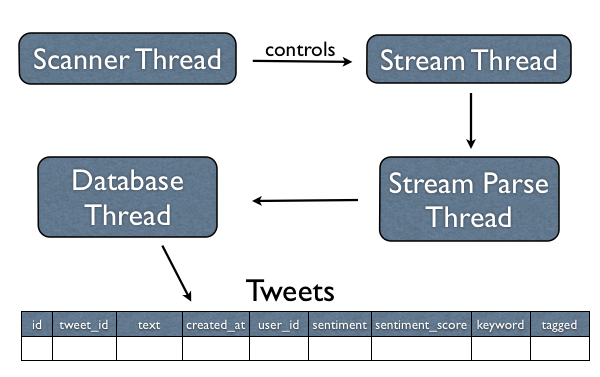
\includegraphics[width=12cm]{tweetir}
\end{center}
\caption{Control flow for tweet retrieval subsystem}
\label{fig:tweetir}
\end{figure}

\begin{lstlisting}[caption=Tweet and User class properties, label=lst:tweetuser]
public class Tweet {
    private final long tweetId;
    private final String tweet;
    private final String createdAt;
    private final User user;
    private String keyword = null; // Only used when filtering
    ...
} // class Tweet

public final class User {
    private final long id;
    private final String username;
    ...
} // class User 
\end{lstlisting}

\begin{figure}[h]
\begin{center}
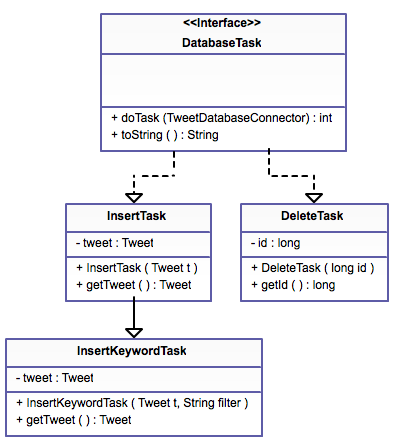
\includegraphics[width=7cm]{dbtask}
\end{center}
\caption{DatabaseTask class diagram}
\label{fig:dbtask}
\end{figure}

\begin{figure}[h]
\begin{center}
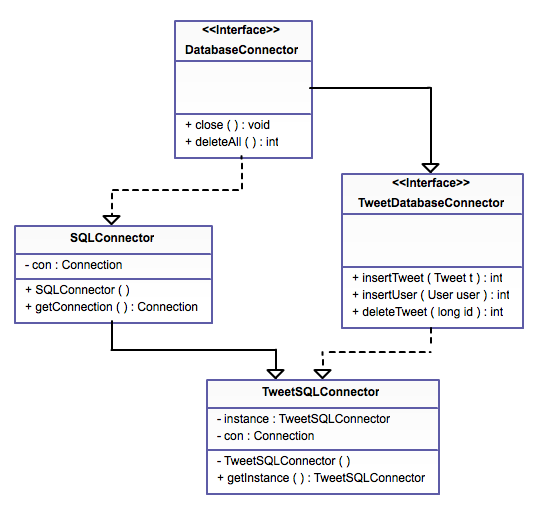
\includegraphics[width=9cm]{dbcon}
\end{center}
\caption{DatabaseConnector class diagram}
\label{fig:dbcon}
\end{figure}

Class design aside, once this \emph{InsertKeywordTask} object has been created, it is added to the queue in the \emph{DatabaseThread}. The respective implementations of the \emph{doTask()} method in each of the DatabaseTask classes will be performed as this queue is emptied. In the case of InsertKeywordTask, this is simply \texttt{db.insertTweet(t)}, where \texttt{db} is the TweetDatabaseConnector passed to it in the \texttt{doTask()} method, and \texttt{t} is the Tweet object it was initialised with.

This process is completed when the \emph{TweetDatabaseConnector} inserts the tweet into the database, in the current implementation using Java Database Connectivity (JDBC) to manipulate the MySQL server.

\subsection{Searching Twitter}
\label{sec:searchjava}
The Search API will now be used to handle use case 2 of the designed system, as described in Section~\ref{sec:uc2}. With the Search API not operating in real time, the realisation of this use case can afford to be a much simpler system. The levels of multithreading displayed in streaming Twitter will not be required, as interaction with the API is more of a serial communication as can be seen in Figure~\ref{fig:ucsearch}.

\begin{figure}[h]
\begin{center}
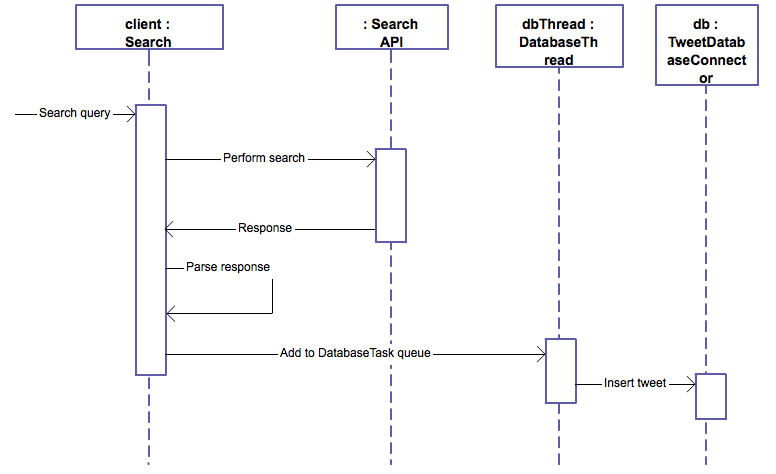
\includegraphics[width=13cm]{ucsearch}
\end{center}
\caption{Searching Twitter sequence diagram}
\label{fig:ucsearch}
\end{figure}

The implementation of the Twitter search use case utilises the Twitter Search API URL at \url{http://search.twitter.com/search.json}. The API also offers eXtensible Markup Language (XML) format responses, however, working with JSON allows consistency within the system. As with the implementation of the Twitter stream use case, the application begins with the initialision of a \emph{DatabaseThread} and is initially given a single keyword which will be searched for. This keyword is chosen by the end user. A simple HTTP GET request is then made to the above URL and Twitter then returns up to 1500 tweets from the last seven days corresponding to the search term.

The Search API returns a different JSON response to that of the Streaming API. Each JSON string contains an \texttt{iso\_language\_code}, and this will be used to filter tweets by language. Once the desired information has been extracted, i.e. the properties of the \emph{Tweet} class, the remaining operations are carried out just as they are in the realisation of the Twitter streaming use case, that is, the tweet is encapsulated in an \emph{InsertKeywordTask} object and this is added to a queue in the \emph{DatabaseThread} for the insert task to be carried out.

% SHOW JSON RESPONSE IN APPENDIX


\python
\section{Feature Extraction}
\label{sec:fe}
Once tweets have been retrieved from Twitter and stored in the MySQL database, they are now available for feature extaction, which can be regarded as the core stage in implementing the system. This subsystem involves using NLP techniques to extract the information described in Section~\ref{sec:arc2} from each tweet. This subsystem is implemented in Python 2.7 due to the raw power it possesses and also due to the decision to use the Natural Language Toolkit (NLTK). It was felt that Python's speed and text manipulation would allow for a better implementation of the system.

There are many steps involved in implementing the feature extraction. These are explored in order of execution.

\subsection{Sentiment Analysis}
Sentiment analysis was recognised as one of the key features to be extracted from the initial design stages (see Figure~\ref{fig:phase2}). It has been implemented using the Sentiment140 Bulk Classification Service API. 
The sentiment analysis of tweets is carried out before any of the other feature extraction work. As tweets have been retrieved and stored in the MySQL database, this part of the system selects the latest tweets, retrieving just the id and text, that have yet to be analysed and packs them into a JSON string object of the format:

\begin{verbatim}
{ "data": [ { "id": "1234", "text": "Google Chrome is awesome!" },
            { "id": "1235", "text": "Safari 5.0.2 is out now" },
            { "id": "1236", "text": "I really hate the new Firefox" } ] }
\end{verbatim}

This JSON string is then posted to the Twitter Sentiment API where classifications into the positive, negative and neutral classes are carried out by a Maximum Entropy classifier, using unigram and bigram features, trained with tweets containing emoticons. The internal specifics of a Maximum Entropy classifier, however, is not in the scope of this project.

Currently only 100 tweets are analysed at a time due to time constraints when users wish to run the program in real time. By using a small number, the data needing to be transferred is minimal and allows for a more interactive user experience.

Using the previous example, the data is returned by the server in the following format, with a polarity field added to each analysed tweet with values 0, 2 and 4 corresponding to negative, neutral and positive respectively.
\begin{verbatim}
{ "data": [ 
  { "id": "1234", "text": "Google Chrome is awesome!", "polarity": 4},
  { "id": "1235", "text": "Safari 5.0.2 is out now", "polarity": 2 },
  { "id": "1236", "text": "I really hate the new Firefox", "polarity": 0 } 
] }
\end{verbatim}

Upon receipt of this response, the JSON formatted string is parsed and the corresponding record for the tweet previously stored in the MySQL database is updated with new values for sentiment score and the actual sentiment, using polarity and its semantic meaning respectively.

\subsection{URL Extraction}
Before extracting context and semantics from tweets, any URLs mentioned are found and removed. Assuming the tweet is software-related, these URLs are quite likely to be links to the software, or further reviews. This task is done using NLTK's \texttt{regexp\_tokenize()} function with \url{http://}\verb/[^ ]+/ passed as the regular expression that finds URLs. If the tweet is later found not to contain any software, these URLs are discarded. Potential issues with this implementation could be that a user may post a URL without the preceding \url{http://} protocol prefix and these would not be found by this regular expression. However, Twitter automatically converts URLs to their \url{http://t.co/} domain and so this is resolved on the Twitter server side.

\subsection{Tokenisation}
After URLs have been extracted and removed from the source text, the tweet is tokenised to produce an array of all the terms in the tweet. The tokenisation process is also done using NLTK's \texttt{regexp\_tokenize()} function, passing it the regular expression - \verb/\w+([.,]\w+)*|\S+/. This expression returned superior results to alternation tokenisation functions provided by NLTK, such as \texttt{wordpunct\_tokenize()} as it was capable of finding numbers and currencies without splitting them. Using the above example,

\begin{quote}
I really hate the new Firefox
\end{quote}
this would be tokenised to the following:
\begin{quote}
[`I', `really', `hate', `the', `new', `Firefox']
\end{quote}

The following example shows a more complicated tokenisation process.
\begin{quote}
Norton Anti-Virus released for \$50 \#ripoff

\begin{math}\Rightarrow\end{math}
[`Norton', `Anti', `-Virus', `released', `for', `\$50', `\#ripoff']
\end{quote}

\subsection{Price Extraction}
\label{sec:price}
Continuing on from this tokenisation of the original source text, the current subsystem attempts to find prices in the array of terms. This is done using Python's built-in regular expression module, \texttt{re}. A number of regular expressions are used to define patterns denoting numbers, currencies and quantifiers like `hundred' and `thousand'. As the form of prices vary, for example in the case of mobile apps you might find `£0.59', `59p' or even `59 pence', these combinations of tokens may be split across two tokens in the array returned from the tokenisation process. For this reason, it is necessary to iterate over all items in the list of tokens while remembering the previous one. This obviously means a less efficient system, however, it has produced the best results in such variable conditions.

\subsection{Part-of-speech (POS) Tagging}
The POS tagger used by this system is taken from the NLTK modules and uses the \texttt{pos\_tag()} function which takes a tokenised sentence as its only argument. Continuing from the first example, this process tags as follows: 
\begin{quote}
[`I', `really', `hate', `the', `new', `Firefox']

\begin{math}\Rightarrow\end{math}
[(`I', `PRP'), (`really', `RB'), (`hate', `JJ'), (`the', `DT'), (`new', `JJ'), (`Firefox', `NNP')]

\begin{center}
\begin{tabular}{ l | l }
  \hline                        
  PRP & Pronoun \\
  RB & Adverb \\
  JJ & Adjective \\
  DT & Determiner \\
  NNP & Proper Noun \\
  \hline  
\end{tabular}
\end{center}
\end{quote}

\subsection{N-Grams}
The implementation of creating n-grams in this project is done using the \texttt{nltk.util.ngrams()} function. This process starts by creating a five-gram of the tweet tokens. This means a sequence of five tokens will be created from the array of tokens. The system utilises a five-gram sequence due to potentially long software names, basing this on the na\"{\i}ve assumption that these names will not exceed five words. This will allow for improved extraction of software names in the next stage. Using the Firefox tweet as a running example, the outcome of this five-gram modelling process can be seen below.

\begin{quote}
[`I', `really', `hate', `the', `new', `Firefox']

\begin{math}\Rightarrow\end{math}

[
 ( (`I', `PRP'), (`really', `RB'), (`hate', `JJ'), (`the', `DT'), (`new', `JJ') ),

 ( (`really', `RB'), (`hate', `JJ'), (`the', `DT'), (`new', `JJ'), (`Firefox', `NNP') )
]
\end{quote}

\subsection{Main Feature Extraction}
This tagging process consists of the core functions of the proposed system. Its purpose is to extract all the features that have yet to be extracted, that is, software names and versions, companies, programming languages and operating systems. It also attempts to find any prices that may previously have been missed, and also has the task of discovering software that is not already in the dictionary.

Having created a set of five-gram sequences from the tweet, the application may now iterate through each of these in an attempt to find any information that has not yet been found. For each of these sequences, the program iterates through each POS-tagged token in the sequence. The tagging process then proceeds as follows: 
\newline
\begin{algorithmic}
\If {token is tagged as a noun}
    \If {token is in dictionary of software, companies, os, programming languages}
        \If {previous token not tagged as determiner or preposition}
            \State Feature has been found
        \EndIf
    \EndIf
\EndIf
\end{algorithmic}

This rule filters out linguistics of the form shown in Figure~\ref{fig:rule1}.
\begin{figure}[h!]
 \centering
  \setlength{\unitlength}{0.0125in}
\begin{picture}(200,10)( 20, 0)
\thicklines
\put(0,0){\framebox(100,20){DETERMINER}}

\put(110,0){\framebox(80,20){SOFTWARE}}

\put(200,0){\framebox(20,20){??}}
\end{picture}

  \caption{A linguistic filter
    \label{fig:rule1}}
\end{figure}
If however, these conditions fail, usually in the case where none of the tokens are in the dictionary of keywords used to retrieve these tweets, a regular expression is used to find clues to the presence of new software.

\begin{quote}
\verb~^download$|^get$~
\end{quote}

The above regular expression matches on the words \emph{download} or \emph{get}. This works on the basis that many tweets about software are usually posted to promote said software. This is generally done by urging others to download it, and that too by means of application stores like the App Store, or Google Play. This then allows the next token to be analysed to check if it is in fact a piece of software. This is done by checking that token's part of speech tag, and if it is a noun, the following tokens are also assessed in case the name of the software is longer than one word. This possible software name is then noted and kept aside for verification by web search as discussed in Section~\ref{sec:bing}. This regular expression can be applied to the five-gram in conjunction with others in order to maximise the number of features extracted. The following expression could be used to find an operating system.

\begin{quote}
\verb~^on$|^for$~
\end{quote}

By applying these together in the form displayed in Figure~\ref{fig:rule2}, the system may be able to determine the platform upon which a piece of software runs.

\begin{figure}[h!]
 \centering
  \setlength{\unitlength}{0.0125in}
\begin{picture}(200,20)( 20, 0)
\thicklines
\put(0,0){\framebox(60,20){Download}}

\put(70,0){\framebox(80,20){SOFTWARE}}

\put(160,0){\framebox(20,20){for}}

\put(190,0){\framebox(20,20){OS}}
\end{picture}

  \caption{A linguistic pattern to find software and the operating system it may run on
    \label{fig:rule2}}
\end{figure}

Once software has been found in the tweet, a search for its version number begins. This essentially works on the assumption that once software has been named, if a version number is to appear, it will be stated either immediately afterwards, or after the word \emph{version}, or some derivative, such as \emph{ver} or \emph{v}.

Finally, this section of the implementation does one more check for prices, this is mainly for free software, as the word \emph{free} would not be found at the price extraction stage explored in Section~\ref{sec:price}. 
\begin{quote}
\verb~^is$|^for$~
\newline
\verb~^free$~
\end{quote}

The above regular expressions are used similarly to the usage of the expression finding operating systems that software may run on. If the first expression is matched in the text, it is likely the next token is a price. In cases where the next token is \emph{free}, it will match the second regular expression, thus signifying the price of the software. This is a na\"{i}ve approach but in most cases the prices will already have been extracted.

This concludes the main feature extraction process leaving just the verification of new software names via a web search. Listings~\ref{lst:extr} and \ref{lst:extr2} show examples of the data structure storing these extracted features.

\begin{lstlisting}[caption=Example of some extracted features, label=lst:extr]
{
  "company_id" : "23",
  "company_name" : "apple",
  "os_id" : "9",
  "os_name" : "ios",
  "software_name" : "ios",
  "tweet" : "There are some new wallpaper in Apple iOS 5.1. Check them out!",
  "tweet_db_id" : "439640",
  "version" : "5.1",
  "sentiment": "positive"
}
\end{lstlisting}

\begin{lstlisting}[caption=Another example of some extracted features, label=lst:extr2]
{
  "price" : "free",
  "software_id" : "159",
  "software_name" : "moodle",
  "tweet" : "Training hundreds or thousands of staff?? If you want easy, affordable e-learning training then download moodle free http://t.co/beZgqaOd",
  "tweet_db_id" : "440065",
  "url" : "http://t.co/beZgqaOd"
}
\end{lstlisting}

\subsection{Software Verification}
\label{sec:bing}
The feature extraction subsystem may discover new software, and as such needs to verify these are actually pieces of software and not something else. To do this the program utilises the Microsoft Bing API which returns web search queries. As the main tagging process checks the dictionary for matching software names, and the tweet retrieval engine uses both the dictionary and a set of keywords, there will be some pieces of software mentioned in the tweets that are not in the dictionary. As a result, these will be flagged as possible software names, and then queried on the Microsoft Bing search engine with the keywords ``movie'', ``music'', and ``software game''. These keywords were selected on the basis that the initial search key terms retrieved many tweets referring to music and films. The implementation of the Bing API integration can be seen in Appendix~\ref{app:bing}.
\newline
\begin{algorithmic}
\Function {bing\_search}{bing, term}
    \State music = bing.search(term, music)
    \State movie = bing.search(term, movie)
    \State software = bing.search(term, software game)
    \newline
    \If {size(software) greater than size(movie) and size(music)}
        \If {references to software in title and description}
            \State \Return True
        \EndIf
    \EndIf
    \newline
    \State \Return False
\EndFunction
\end{algorithmic}
If the number of results for software associated with the searched term is greater than corresponding results for films and music, the results are checked for identifiers of software in their headings. Therefore if any of the results suggests the searched term is a piece of software, that is assumed true.

\section{Storing the Extracted Information}
As the information being extracted is temporarily stored in a Python dictionary variable, it is essentially in the form of a JSON string. The database design for storing this information is also in the form of a NoSQL database. For this reason, a document-based database system seems to be the best approach. By using MongoDB, it is easy to store the extracted information, as it is as straightforward as directly storing the string representation of this variable as a record in the database. Once this information has been successfully stored in MongoDB, the boolean \emph{tagged} flag is set to True for the corresponding tweet in the MySQL database.

\section[Visualisation]{Visualisation/Graphical User Interface(GUI)}
The final stage of the project is to aggregate and present the results to the user in a GUI.

\subsection{Aggregation}
The aggregation process has been implemented in Python because the MongoDB wrapper class has already been written and due to the simple mapping between Python dict types and MongoDB's stored documents.

This stage involes two processes. The first of these is finding the general sentiment towards a particular piece of software from all of the tweets mentioning said software, as in use case 3 (Section~\ref{sec:uc3}). This is a simple \emph{find} query and the command and syntax for carrying out this task in Python is equivalent to its MongoDB counterpart. The following command would retrieve documents containing the key-value pair of \texttt{software\_name=firefox}, given the collection, MongoDB's equivalent of a table in a relational database, is named \texttt{tagged\_tweets}.
\begin{quote} 
\begin{lstlisting}
db.tagged_tweets.find( { `software_name': `firefox' } )
\end{lstlisting}
\end{quote}

Upon retrieving these documents, the application extracts the distinct values from the \texttt{sentiment} field of each document, which can be \emph{positive}, \emph{negative} or \emph{neutral}. For each of these values that appears, its appearance count is calculated using a looping function and these counts are used to make charts in the web application, the topic of discussion in Section~\ref{sec:webapp}.

The second task, use case 4 (Section~\ref{sec:uc4}), is to find the top tweeted software and also includes operating systems in the final implementation. This is completed using a grouping function defined in the Python MongoDB driver module.

\begin{quote}
\begin{lstlisting}
def _group(self, key):
        return self.tags.group(key=[key],
                               condition={key:{`\$ne':None}},
                               initial={`count':0},
                               reduce=`function(obj,prev) { prev.count += 1;}')
\end{lstlisting}
\end{quote}

The above function returns a list of items grouped by a given \texttt{key}. The items in the list are also given a \texttt{count} value which is the number of times that software name will have appeared in the database collection. This list is then sorted in descending order and a slice of the top ten of these results are returned to be displayed to the user.

\subsection{Web Application}
\label{sec:webapp}
The web application is required to work with both the Python and the Java code in this project. As such, a static web page is far from the desired solution. This leaves the options of a Java web servlet or a Python web application. Both of these are good options, however, running a Python interpreter inside the Java Virtual Machine(JVM) is a much slower process than invoking Java classes from Python. This can be done using Jython, a Python implementation for Java that allows developers to both invoke Java from Python and vice versa \cite{Juneau:2010}. An alternative solution is to run shell commands directly through the Python interpreter in order to run the Java classes. This is the chosen route of action because no information needs to be passed between the two platforms that cannot be sent as command-line arguments when running the Java code.

Now that this has been decided, a Python web framework must be chosen for the development of this GUI. The CherryPy web framework was selected ahead of the likes of Django and Pylons due to its simplicity and pythonic interface \cite{cherrypy}. For an appealing web design that is easy to create, a templating language must be used to embed Python code. This will be done using the Mako template library\footnote{\url{http://www.makotemplates.org/}}. Mako is a leading templating library that is used by some major websites, such as \url{python.org} itself. Mako was chosen ahead of others such as Genshi, which is an XML-based templating engine, as its syntax is much more similar to that of normal Python code. Mako templates also support inheritance as can be seen in Listing~\ref{lst:mako} provided in Appendix~\ref{app:webapp}. HTML5, CSS and the JavaScript library jQuery make up the rest of the web development environment.

As designed, the web application has to carry out three functions, corresponding to use cases 2, 3 and 4, as described in Section~\ref{sec:uc}. Users must be able to \textbf{search} Twitter, \textbf{analyse} stored results and \textbf{view} the top tweeted operating systems and software. The first of these tasks, the search, is carried out using the Java implementation of integrating Twitter's Search API. Python's \texttt{subprocess} module allows shell commands to be executed inside the Python interpreter. This feature is exploited to run the \\\texttt{uk.ac.manchester.cs.patelt9.twitter.SearchAPI} class, its implementation details explored in Section~\ref{sec:searchjava}, and check its output in the shell. This output is piped through to the web application and finally displayed on the web page. This is shown in Chapter~\ref{cha:results} when discussing the results of the project.

The user may then opt to follow through the entire feature extraction process. By restricting the search to a fairly small number of tweets, this process is heavy in terms of time consumption. By opting to do so, the user allows the application to check the sentiment of each of the tweets, and then follow through the feature extraction process described in Section~\ref{sec:fe}. At the end of this extraction, all the new information is returned in the form of a list, ready for display on the web page.

The next task is to show the user the results that have already been stored in the database. As per the design, this is done by showing the user a drop down menu consisting of all of the software that exists in the database. Upon selecting from the list, the application uses the aggregation methods described in the previous section to retrieve sentiment data. These are then used as input to the Google Chart Tools API, which creates pie charts displaying percentages for each distinct sentiment value.

Finally, the web application's home page shows a list of the top ten most tweet operating systems and software as links to the charts of these tools. This is again done using the aggregation methods set up in the previous stage of implementation.

\section{Testing}
Due to the agile approach taken in the development of the SWOT system, testing was carried out iteratively throughout the project. This was done in the form of unit and integration tests. Unit testing refers to tests that verify code modules or class function properly. These tests were performed throughout implementation to ensure each core stage was fully functional, particularly in the feature extraction phase. For example, in the price extraction process, the string ``\$8 million '' should return the full string as a price whereas ``8 million'' should yield a negative price match.

Integration testing is performed when any two fully tested units are combined to create a larger structure. This was also carried out throughout development but was most apparent when implementing SWOT's web application. The web application required the integration of every other Python function developed as well as the Java implementation of the Twitter search use case. For optimal user experience, these independent functions must integrate seamlessly to appear transparent to the user.

System tests were performed towards the end of the implementation of the system in order to verify the initial requirements stated in the design phase (see Chapter~\ref{cha:design}) have been met. In SWOT's case, this is essentially ensuring all of the specified features have been extracted from tweets where possible, and further details have been provided on this stage in Chapter~\ref{cha:results}, where results have been detailed.


\chapter{Results}
\label{cha:results}
This chapter details the results of the project, along with views of the user interface and the final findings of the system.

\section{GUI}

\begin{figure}[h]
\begin{center}
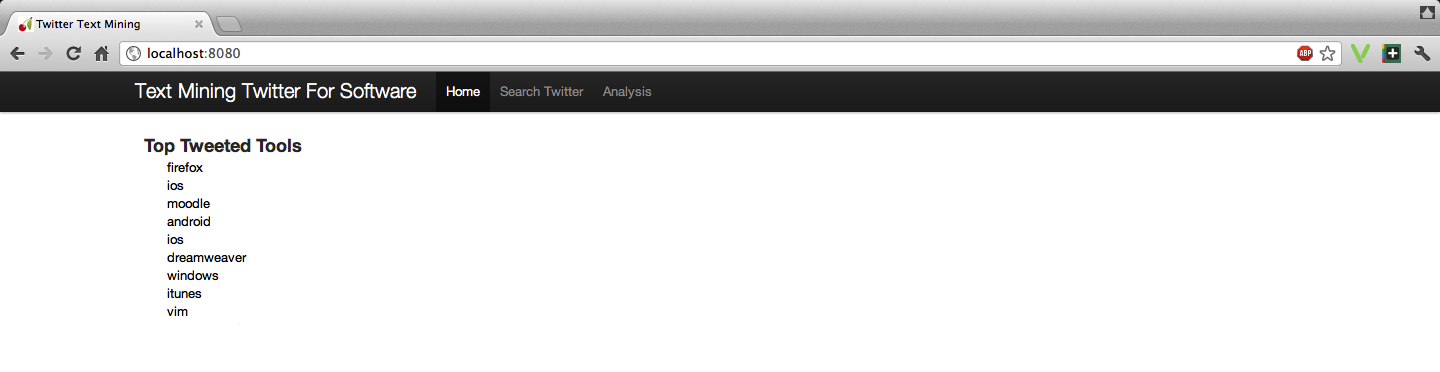
\includegraphics[width=15cm]{gui1}
\end{center}
\caption{The web application's home page}
\label{fig:gui1}
\end{figure}


\begin{figure}[h]
\begin{center}
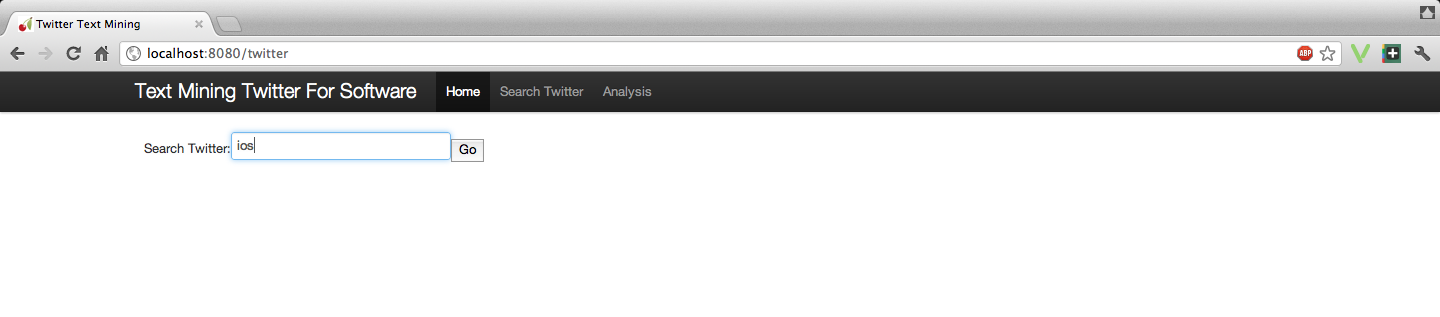
\includegraphics[width=15cm]{gui2}
\end{center}
\caption{The web application's search page}
\label{fig:gui2}
\end{figure}

\begin{figure}[h]
\begin{center}
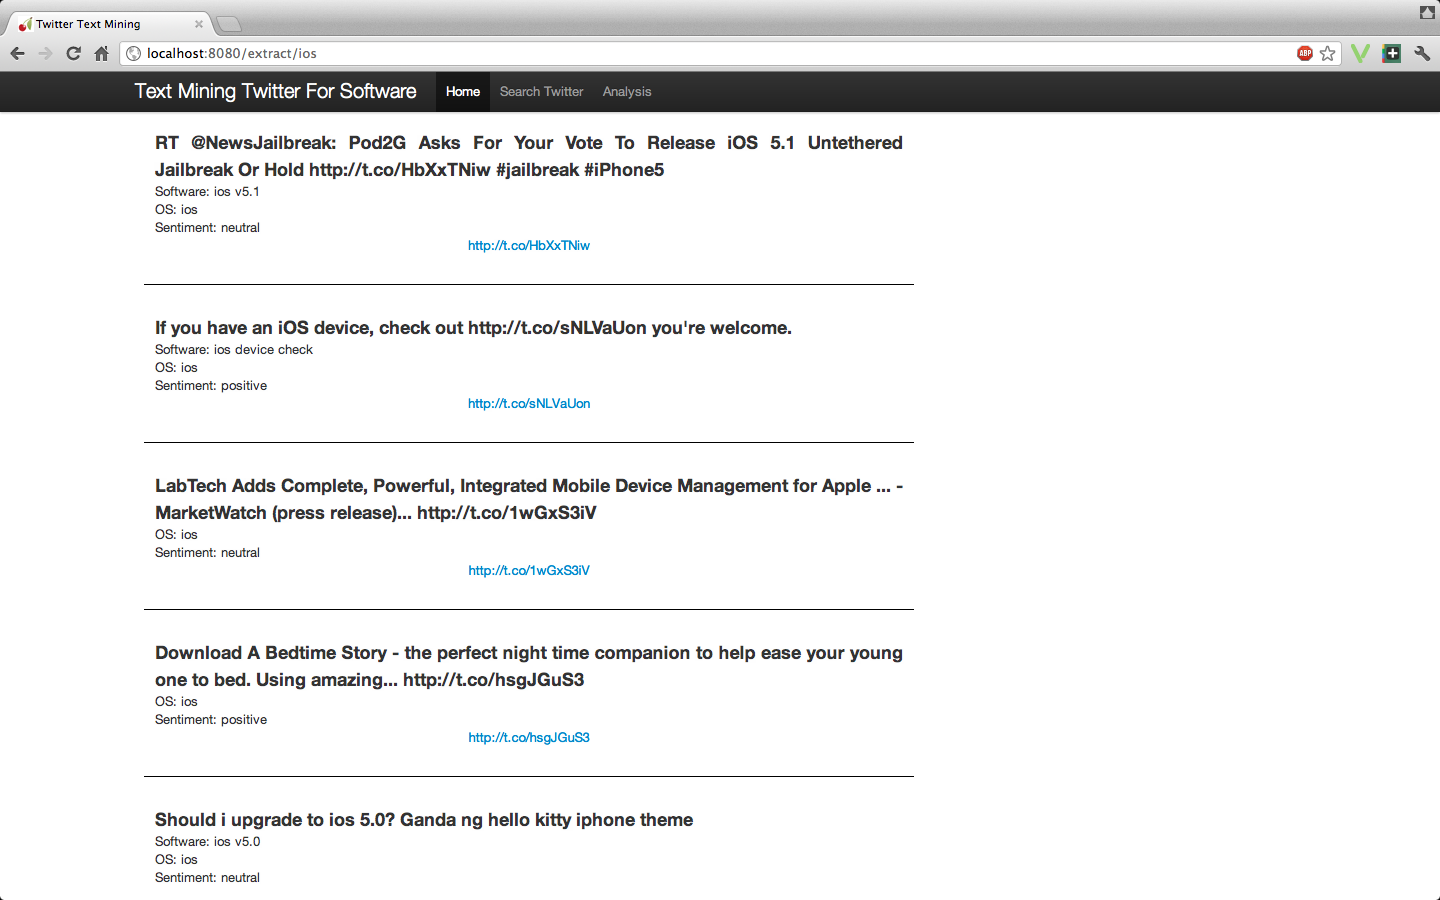
\includegraphics[width=15cm]{gui3}
\end{center}
\caption{The web application's extracted features page}
\label{fig:gui3}
\end{figure}


\begin{figure}[h]
\begin{center}
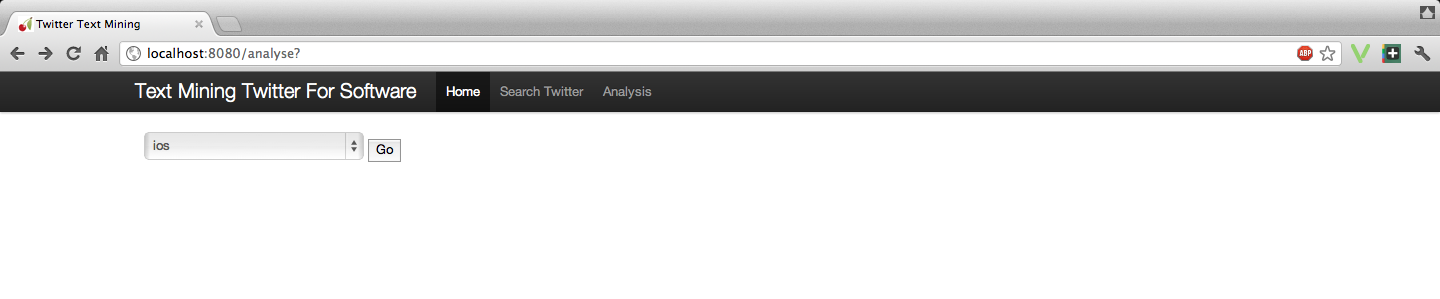
\includegraphics[width=15cm]{gui4}
\end{center}
\caption{The web application's analysis dropdown menu}
\label{fig:gui4}
\end{figure}

\begin{figure}[h]
\begin{center}
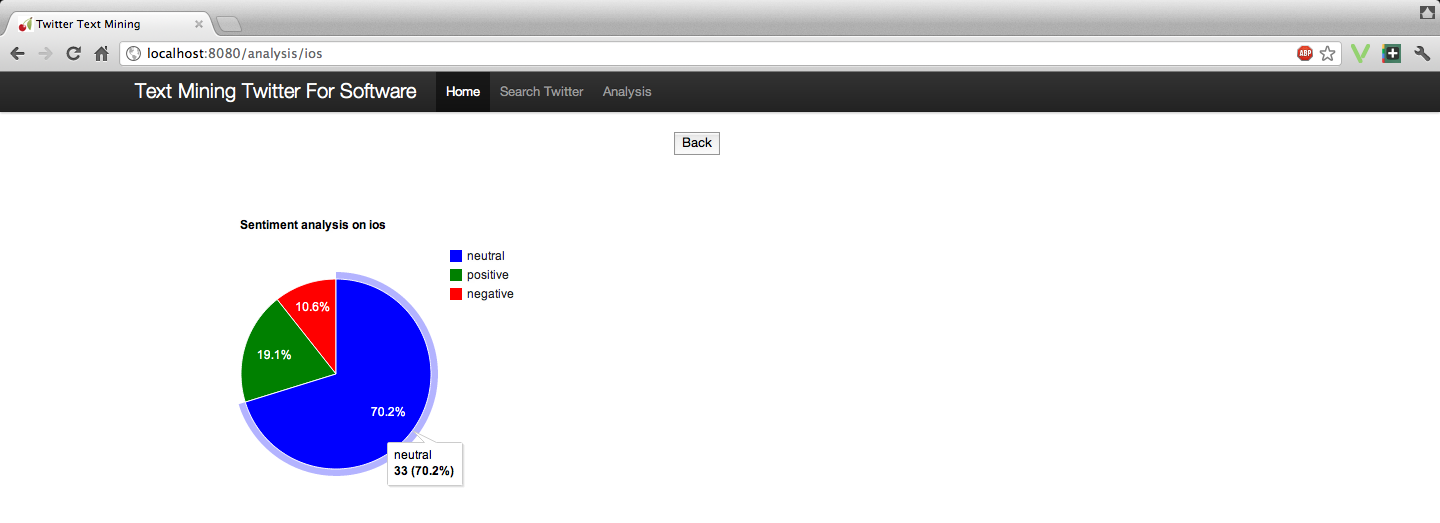
\includegraphics[width=15cm]{gui5}
\end{center}
\caption{The web application's analysis page for a specified piece of software}
\label{fig:gui5}
\end{figure}

% gui screenshots
\section{Discussion}

\chapter{Evaluation}
\label{cha:eval}
With implementation and analysis complete, one can now identify and evaluate the key successes and shortcomings of this project. These evaluations have been performed on the basis of the following questions:

\begin{itemize}
\item Does the system work?
\item Is the information found novel and interesting?
\item Is the system easy to use?
\end{itemize}

This process has been carried out by means of independent user evaluations by 5 users of the software.
\chapter{Conclusions}
\label{cha:conclusion}
This chapter discusses the author's reflections on the success and conclusions of the project. Suggestions for further work are made and concludes with a summary of the report. 

\section{Reflections}
In terms of the overall progress made over the course of the year I feel this project has to some extent been a success. It has been a steep learning curve and on that basis some good results have been achieved. However, in absolute terms, I think I have made many mistakes in the way I went about working on the project over the year. This is down to a few key issues.

\textbf{Time management} can be seen as one of the overriding causes of the shortfalls of this project. There were times when progress had completely stalled due to minor issues with implementation.
%eg dictionary


I also feel as though my \textbf{preparation} may not have been sufficient, as I had overlooked a few key concepts when developing parts of the system. For example, I did not create a training set of data that would ultimately allow me to use a machine learning approach in my system and I think this may have resulted in a slightly lesser performing program, in terms of its accuracy.

% MORE ISSUES HEE


However, as previously stated, there have been major strides over the year. I feel I have a much greater grounding in the core object oriented design and programming principles. As well as this, I have developed skills in many new technologies and concepts. This was the first time I have had to develop a multithreaded desktop environment, and I had never previously worked with Python, JSON, MongoDB or the HTTPS protocol. As such I am happy with the general progress made in this project.

\section{Future Work}
%futurework - word frequencies
% reason behind tweet



\nocite{*}
\bibliography{refs}             % this causes the references to be
                                % listed

\bibliographystyle{alpha}       % this determines the style in which
                                % the references are printed, other
                                % possible values are plain and abbrv
%% Appendices start here
\appendix
\chapter{Dictionary of Software and Keywords}
\label{app:dictionary}

\begin{table}[h]
\begin{center}
\begin{tabular}{|l|l|l|}\hline
software&app&mac\\\hline
pc&alpha&beta\\\hline
version&source code&sdk\\\hline
release&api&version\\\hline
game&&\\\hline
\end{tabular}
\end{center}
\caption{List of keywords}
\end{table}

\begin{table}[h]
\begin{center}
\begin{tabular}{|l|l|l|}\hline
Apache&Mozilla&Activision\\\hline
Infinity Ward&Blizzard&EA\\\hline
Rockstar Games&HP&Codemasters\\\hline
Valve&Adobe&Blackberry\\\hline
Cisco&SlingMedia&Maxis\\\hline
Rarlabs&VideoLan&ATI\\\hline
Atari&Symantec&Nvidia\\\hline
Oracle&Apple&Microsoft\\\hline
Google&&\\\hline
\end{tabular}
\end{center}
\caption{Dictionary of companies}
\end{table}

\begin{table}[h]
\begin{center}
\begin{tabular}{|l|l|l|}\hline
WebOS&Android&Bada\\\hline
Symbian&Linux&Fedora\\\hline
Ubuntu&Windows&iOS\\\hline
OS X&MacOS&FreeBSD\\\hline
\end{tabular}
\end{center}
\caption{Dictionary of operating systems}
\end{table}


\begin{table}
\begin{center}
\begin{tabular}{|l|l|l|}\hline
ZeuAPP&Bitcoin&vtiger CRM\\\hline
ReOS&SugarCRM&OrangeHRM\\\hline
Ebase&Dolibarr ERP/CRM&Bonita Open Solution\\\hline
Adempiere&bookyt&Compiere\\\hline
FrontAccounting&GnuCash&Grisbi\\\hline
HomeBank&jFin&JFire\\\hline
JGnash&JQuantLib&KMyMoney\\\hline
LedgerSMB&MibianLib&Mifos\\\hline
Octopus Micro Finance Suite&Openbravo&OpenERP\\\hline
Postbooks&QuickFIX&QuickFIX/J\\\hline
SQL Ledger&Tryton&TurboCASH\\\hline
WebERP&refbase&Koha\\\hline
NewGenLib&OpenBiblio&PMB\\\hline
SimPy&CellProfiler&ImageJ\\\hline
Endrov&Jmol&Molekel\\\hline
MeshLab&PyMOL&QuteMol\\\hline
RasMol&Avogadro&Ascalaph Designer\\\hline
GROMACS&LAMMPS&MDynaMix\\\hline
NAMD&Chemistry Development Kit&JOELib\\\hline
OpenBabel&P-GRADE Portal&OpenCog\\\hline
OpenCV&AForge.NET&ROS\\\hline
TREX&CMU Sphinx&Emacspeak\\\hline
Festival Speech Synthesis System&NVDA&Text2Speech\\\hline
NonVisual Desktop Access&ESpeak&Dasher\\\hline
Gnopernicus&Virtual Magnifying Glass&OpenAFS\\\hline
Eucalyptus&AppScale&FusionCharts\\\hline
ParaView&Orange&RapidMiner\\\hline
Scriptella ETL&Weka&jHepWork\\\hline
Konstanz Information Miner&KNIME&ELKI\\\hline
Lucene&Solr&Xapian\\\hline
Nutch&CloverETL&Talend\\\hline
Pentaho&SpagoBI&Limesurvey\\\hline
OpenX&RSS Bandit&RSSOwl\\\hline
Akregator&Liferea&Ekiga\\\hline
\end{tabular}
\end{center}
\caption{Dictionary of software}
\end{table}
\begin{table}
\begin{center}
\begin{tabular}{|l|l|l|}\hline
FreePBX&FreeSWITCH&Jitsi\\\hline
QuteCom&sipX&Slrn\\\hline
FreeNX&OpenVPN&rdesktop\\\hline
VNC&RealVNC&TightVNC\\\hline
UltraVNC&xrdp&HTTrack\\\hline
Wget&Apache Cocoon&AWStats\\\hline
BookmarkSync&CougarXML&curl-loader\\\hline
HTTP File Server&Distributed ICDL Crawler&Crawley Framework\\\hline
lighttpd&nginx&NetKernel\\\hline
Piwik&Qcodo&Web-Developer Server Suite\\\hline
XAMPP&Zope&Oxwall\\\hline
Liferay&Sun Java System Portal Server&uPortal\\\hline
Apache Axis2&Apache Geronimo&GlassFish\\\hline
CORBA&JacORB&Jakarta Tomcat\\\hline
JBoss&ObjectWeb JOnAS&OpenSplice DDS\\\hline
SmartVariables&OpenLDAP&JXplorer\\\hline
openVXI&YaCy&Gnaural\\\hline
DoceboLMS&eFront&GCompris\\\hline
IUP&Moodle&Omeka\\\hline
Sakai&Chamilo&openSIS\\\hline
ATutor&ILIAS&Kiten\\\hline
KVerbos&KTouch&KGeography\\\hline
KEduca&openlp.org&BibleDesktop\\\hline
BibleTime&Xiphos&SWORD Project\\\hline
SwordBible&Go Bible&jSword\\\hline
MacSword&Marcion&Eye of GNOME\\\hline
F-spot&Gqview&Gthumb\\\hline
imgSeek&Kphotoalbum&Dream DRM Receiver\\\hline
KToon&Synfig&K-3D\\\hline
OpenFX&Seamless3d&Pencil Animation\\\hline
SWFTools&Avidemux&AviSynth\\\hline
Blender&Cinelerra&CineFX\\\hline
Jahshaka&DScaler&DVD Flick\\\hline
\end{tabular}
\end{center}
\caption{Dictionary of software}
\end{table}
\begin{table}
\begin{center}
\begin{tabular}{|l|l|l|}\hline
DVDx&Kaltura&Kino\\\hline
Kdenlive&OpenShot Video Editor&PiTiVi\\\hline
VirtualDub&VirtualDubMod&Celtx\\\hline
KeePass&Password Safe&TeamLab\\\hline
Project.net&KAddressBook&Kontact\\\hline
KOrganizer&Novell Evolution&OpenSync\\\hline
Rachota Timetracker&Bugzilla&Mindquarry\\\hline
Redmine&Trac&Open Scene Graph\\\hline
OpenSCDP&CodeSynthesis XSD&CodeSynthesis XSD/e\\\hline
xmlbeansxx&Flex lexical analyser&Kodos\\\hline
phpCodeGenie&\^txt2regex\$&SableCC\\\hline
Autoconf&Automake&Xnee\\\hline
Memtest86&JSystem&GNU Debugger\\\hline
ClamAV&ClamWin&Gateway Anti-Virus\\\hline
AVG antivirus&Winpooch&MyDLP\\\hline
GnuPG&KGPG&Seahorse\\\hline
GnuTLS&OpenSSL&CrossCrypt\\\hline
FreeOTFE and FreeOTFE Explorer&Iptables&Coyote Linux\\\hline
Firestarter&IPFilter&ipfw\\\hline
IPCop&IPFire&M0n0wall\\\hline
PeerGuardian&pfSense&SmoothWall\\\hline
Shorewall&Untangle&Vyatta\\\hline
Zentyal&Lsh&OpenSSH\\\hline
PuTTY&Cyberduck&Agorum\\\hline
Anti-Spam SMTP Proxy&Balsa&Bogofilter\\\hline
Citadel/UX&Claws Mail&Dada Mail\\\hline
DSPAM&Enigmail&Exim\\\hline
Fdm&Fetchmail&FreePOPs\\\hline
FUDforum&Getmail&GNUMail\\\hline
Gnus&Gnuzilla&GPGMail\\\hline
GroupServer&Hypermail&I-sense\\\hline
IlohaMail&Internet Messaging Program&Libremail\\\hline
GNU Mailman&MailScanner&Mailx\\\hline
\end{tabular}
\end{center}
\caption{Dictionary of software}
\end{table}
\begin{table}
\begin{center}
\begin{tabular}{|l|l|l|}\hline
Majordomo&MH Message Handling System&MIMEDefang\\\hline
Movemail&Mozilla Mail&Mozilla Thunderbird\\\hline
Mutt&NeoMail&Open-Xchange\\\hline
POPFile&Qpopper&Roundcube\\\hline
Scalix&SimpleMail&Smail\\\hline
Smartlist&SpamAssassin&Spicebird\\\hline
SquirrelMail&Sylpheed&Sympa\\\hline
Uebimiau&Universal village collaboration suite&UW IMAP\\\hline
Vpopmail&Xuheki&Yet Another Mailer\\\hline
YPOPs!&Zarafa&Zimbra\\\hline
Adium&AMSN&Ayttm\\\hline
BitlBee&Bombus&Bombusmod\\\hline
Centericq&Climm&Coccinella\\\hline
Emesene&Fama IM&Gabber\\\hline
Gajim&Instantbird&JabberMixClient\\\hline
Jimm&JWChat&Kadu\\\hline
Kopete&Meetro&Miranda IM\\\hline
Monal&Naim&Neustradamus\\\hline
Pandion&Pidgin&Proteus\\\hline
Retroshare&SFLphone&Tapioca\\\hline
TerraIM&Tkabber&Tmsnc\\\hline
TorChat&Zephyr&uTorrent\\\hline
Skype&Sopcast&Spotify\\\hline
Google Chrome&Steam&TextMate\\\hline
Text Editor&TextEdit&nedit\\\hline
gedit&BitLord&bittorrent\\\hline
iTunes&AVG&MS Office\\\hline
f.lux&WinRar&VLC\\\hline
Radeon&Daemon tools&iTunes Match\\\hline
emacs&Firefox&Dreamweaver\\\hline
\end{tabular}
\end{center}
\caption{Dictionary of software}
\end{table}



\end{document}
